\documentclass[11pt]{article}

\usepackage[T1]{fontenc}
\usepackage{lmodern}
\usepackage[margin=1in]{geometry}
\usepackage{amsmath,amssymb,amsthm}
\usepackage{mathtools}
\usepackage{enumitem}
\usepackage{booktabs}
\usepackage{xcolor}
\usepackage{tikz}
\usetikzlibrary{positioning,arrows.meta,fit}
\usepackage[colorlinks=true,linkcolor=blue,citecolor=blue,urlcolor=blue]{hyperref}

% ---------- palette (matches the project site and slides) ----------
\definecolor{ink}{RGB}{24,32,40}
\definecolor{trust}{RGB}{21,110,84}
\definecolor{agent}{RGB}{70,84,156}
\definecolor{flag}{RGB}{179,55,43}
\definecolor{muted}{RGB}{90,100,114}
\definecolor{paper}{RGB}{246,247,244}
\definecolor{trustwash}{RGB}{233,242,236}
\definecolor{agentwash}{RGB}{237,239,248}

\newcommand{\GF}{\mathbb{F}_2}
\newcommand{\HX}{H_X}
\newcommand{\HZ}{H_Z}
\newcommand{\rank}{\operatorname{rank}}
\newcommand{\wt}{\operatorname{wt}}
\newcommand{\supp}{\operatorname{supp}}
\newcommand{\diam}{\operatorname{diam}}
\newcommand{\eff}{kd^2/n}

\title{\textbf{The QEC Challenge}\\[4pt]
	\large A public, automatically verified leaderboard for quantum
	low-density parity-check codes}
\author{Unitary Foundation \and
	\texttt{github.com/unitaryfoundation/qldpc-challenge}}
\date{\vspace{-2ex}\today}

\begin{document}
	\maketitle

	\begin{abstract}
		The QEC Challenge is a public leaderboard for quantum low-density
		parity-check codes. A participant submits a single JSON file describing
		one CSS code; continuous integration recomputes the code's properties
		and actively tries to refute its distance claim, and only a code that
		holds up is merged onto the board. Three principles shape the design.
		(i) \emph{Everything cheap is trustless and mandatory}: the verifier
		recomputes $n$, $k$, CSS commutation, check weight, and the geometric
		locality class from scratch over $\GF$ --- a wrong claimed $k$ or a
		non-commuting ``stabilizer'' is rejected in milliseconds. (ii)
		\emph{Distance is layered by how much is proven}: a submitter attaches
		an explicit logical-operator \emph{witness} that proves
		$d\le\text{value}$ with no trust required; an adversarial
		\emph{refutation gate} then searches for a lighter logical, and
		separate certification tiers upgrade a claim to \emph{corroborated} or
		\emph{exact}. (iii) \emph{A code is not a single number}: the primary
		tracks are a grid of two \emph{computed} axes (locality class $\times$
		check-weight class), and within each cell the ranking is a Pareto
		frontier over $(n,k,d,w)$ rather than a scalar. The whole pipeline ---
		validator, refutation gate, exact certifier, scorer, static-site
		generator --- lives in the repository and runs in CI on every pull
		request, which also makes the board usable as the verification harness
		of automated (LLM- and agent-driven) code-discovery loops.
	\end{abstract}

	\section{Overview}

	A submission is one JSON file placed under \texttt{codes/}, conforming to
	\texttt{schema/code.schema.json} (described in \texttt{schema/SCHEMA.md}). A
	contributor opens a pull request adding the file (one new code per PR,
	enforced by CI); GitHub Actions runs the verifier
	(\texttt{verify/qldpc\_verify.py}) and the distance refutation gate
	(\texttt{verify/gate\_changed.py}), and a green check means the code's
	cheap properties are confirmed \emph{and} an adversarial search failed to
	find a logical lighter than the claimed distance. After merge,
	\texttt{site/build.py} regenerates the static leaderboard into
	\texttt{docs/} automatically (an index with per-cell Pareto tables and
	plots, a page per code, a reference list, and status badges). The board is
	seeded with literature baselines --- the planar open-boundary codes of
	Liang, Eberhardt, and Chen~\cite{liang2025planar}, the bivariate-bicycle
	gross code~\cite{bravyi2024high}, generalized-bicycle
	codes~\cite{panteleev2021degenerate,wang2022distance}, coset
	codes~\cite{aydin2026breaking}, and the surface, toric, and Steane
	codes~\cite{kitaev2003fault,steane1996error} --- so a new entry is always measured against published
	codes rather than an empty board.

	Two things are deliberately \emph{not} asked of the submitter: a proof
	that their distance is exact (that is the server's job), and a single
	headline rank (the board is a Pareto frontier). Everything else --- the
	parity checks, the claimed $n,k,d$ with witnesses, an optional layout, and
	provenance --- is supplied and then recomputed, witnessed, or attacked by
	the verifier.

	\begin{figure}[h]
	\centering
	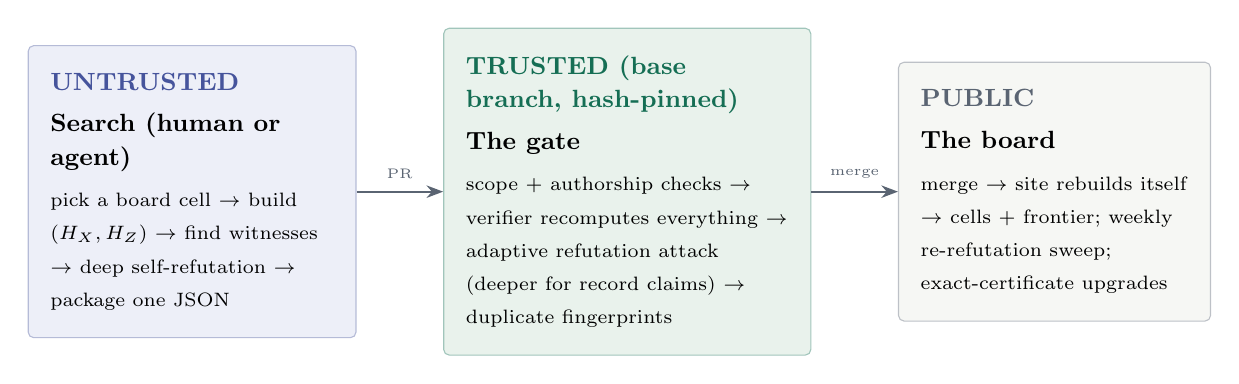
\begin{tikzpicture}[
		zone/.style={rounded corners=2pt, inner sep=8pt},
		arr/.style={-{Stealth[length=6pt]}, thick, muted}]
		\node[zone, fill=agentwash, draw=agent!40] (a) at (0,0)
			{\begin{minipage}{3.6cm}\raggedright\vspace{2pt}
			{\color{agent}\bfseries\small UNTRUSTED}\\[3pt]
			{\bfseries\small Search (human or agent)}\\[3pt]
			{\scriptsize pick a board cell $\to$ build $(\HX,\HZ)$ $\to$
			 find witnesses $\to$ deep self-refutation $\to$
			 package one JSON}\vspace{2pt}\end{minipage}};
		\node[zone, fill=trustwash, draw=trust!40, right=1.1cm of a] (b)
			{\begin{minipage}{4.1cm}\raggedright\vspace{2pt}
			{\color{trust}\bfseries\small TRUSTED (base branch, hash-pinned)}\\[3pt]
			{\bfseries\small The gate}\\[3pt]
			{\scriptsize scope + authorship checks $\to$ verifier recomputes
			 everything $\to$ adaptive refutation attack (deeper for record
			 claims) $\to$ duplicate fingerprints}\vspace{2pt}\end{minipage}};
		\node[zone, fill=paper, draw=muted!40, right=1.1cm of b] (c)
			{\begin{minipage}{3.4cm}\raggedright\vspace{2pt}
			{\color{muted}\bfseries\small PUBLIC}\\[3pt]
			{\bfseries\small The board}\\[3pt]
			{\scriptsize merge $\to$ site rebuilds itself $\to$ cells +
			 frontier; weekly re-refutation sweep; exact-certificate
			 upgrades}\vspace{2pt}\end{minipage}};
		\draw[arr] (a) -- node[above=1pt, font=\tiny, muted] {PR} (b);
		\draw[arr] (b) -- node[above=1pt, font=\tiny, muted] {merge} (c);
	\end{tikzpicture}
	\caption{Three zones, one direction of trust. A submission originates in
	an untrusted search (increasingly, an automated one), is judged entirely
	by pinned code running from the base branch, and only then becomes part of
	the public record --- which keeps being re-attacked after merge.}
	\label{fig:zones}
	\end{figure}

	\section{Why a leaderboard of cells, not one number}

	A quantum code trades several quantities against one another --- physical
	qubits $n$, logical qubits $k$, distance $d$, maximum check weight $w$, and
	geometric locality --- and separately has a decoding performance.
	Collapsing all of that into one scalar would reward gaming one axis at the
	expense of the rest. So the board is stratified in three layers
	(\texttt{TRACKS.md}).

	\paragraph{Layer 1: primary tracks, computed, never self-declared.} The
	primary tracks are a grid of two nested axes whose membership is
	\emph{derived by the verifier} from the parity checks and the layout, so a
	track cannot be claimed by relabeling:
	\begin{itemize}[nosep]
		\item a \textbf{locality class}: \texttt{local-2d-single} (one layer,
		interaction radius $\le 4$) $\subset$ \texttt{local-2d-bilayer} (up to
		two layers --- the flip-chip regime --- radius $\le 7$) $\subset$
		\texttt{unrestricted} (everything else, including any code without a
		layout);
		\item a \textbf{check-weight class}: \texttt{weight-4} $\subset$
		\texttt{weight-6} $\subset$ \texttt{weight-8} $\subset$ any weight,
		from the maximum row weight of $\HX,\HZ$.
	\end{itemize}
	The classes nest: a single-layer weight-4 code also competes on every
	looser board. Each (locality, weight) cell is a board of its own
	(Figure~\ref{fig:grid}).

	\begin{figure}[h]
	\centering
	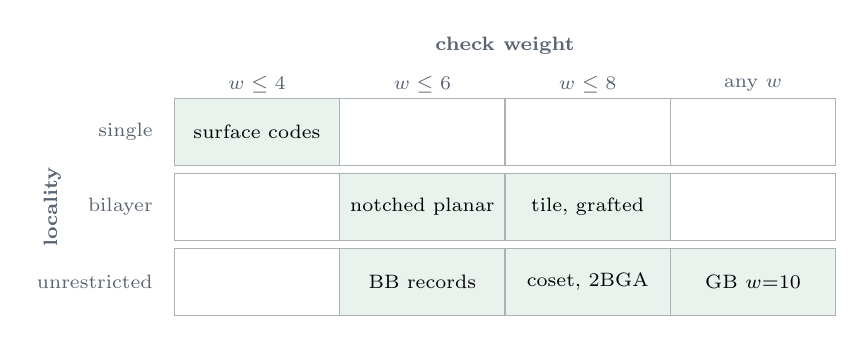
\begin{tikzpicture}[
		cell/.style={draw=muted!50, minimum width=2.1cm, minimum height=0.85cm,
		             font=\scriptsize, inner sep=2pt}]
		\node[font=\scriptsize\bfseries, muted] at (3.15, 3.0) {check weight};
		\foreach \j/\wl in {0/{$w\le4$}, 1/{$w\le6$}, 2/{$w\le8$}, 3/{any $w$}}
			\node[font=\scriptsize, muted] at (2.1*\j, 2.5) {\wl};
		\node[font=\scriptsize\bfseries, muted, rotate=90] at (-2.6, 0.95) {locality};
		\foreach \i/\ll in {0/{single}, 1/{bilayer}, 2/{unrestricted}}
			\node[font=\scriptsize, muted, anchor=east] at (-1.2, 1.9-0.95*\i) {\ll};
		\foreach \j in {0,...,3} \foreach \i in {0,...,2}
			\node[cell] at (2.1*\j, 1.9-0.95*\i) {};
		\node[cell, fill=trustwash] at (0, 1.9) {surface codes};
		\node[cell, fill=trustwash] at (2.1, 0.95) {notched planar};
		\node[cell, fill=trustwash] at (4.2, 0.95) {tile, grafted};
		\node[cell, fill=trustwash] at (2.1, 0.0) {BB records};
		\node[cell, fill=trustwash] at (4.2, 0.0) {coset, 2BGA};
		\node[cell, fill=trustwash] at (6.3, 0.0) {GB $w{=}10$};
	\end{tikzpicture}
	\caption{The primary-track grid: locality class $\times$ check-weight
	class, both computed from the submission (example occupants shown).
	Within each cell the ranking is the Pareto frontier over $(n,k,d,w)$; a
	code in a tight cell also competes in every looser cell it nests into.}
	\label{fig:grid}
	\end{figure}

	\paragraph{Layer 2: family tags, filterable, never ranked.} The
	construction family (bivariate bicycle, generalized bicycle --- including
	non-abelian two-block group-algebra
	constructions~\cite{lin2024quantum} --- coset, tile, topological,
	\dots) cannot be recovered from the matrices, so it is a
	self-reported, filterable tag that confers no ranking advantage.

	\paragraph{Layer 3: verified flags.} Only properties a verifier or a
	certificate can prove: CSS commutation, the locality class (which doubles
	as Layer-1 membership), and the distance-confidence tier of
	Section~\ref{sec:distance}.

	\paragraph{Pareto frontier, not a single winner.} Within a cell, a code is
	a record if no other code in the cell dominates it --- no other has
	$n'\le n$, $k'\ge k$, $d'\ge d$, $w'\le w$ with at least one strict
	inequality. There can be many co-leaders.

	\paragraph{$\eff$ as a sortable column, not the rank.} The
	encoding-efficiency figure $\eff$ used by the 2D-locality literature is
	reported per cell and sortable, but it never collapses the frontier into
	one number.

	\section{Background: the $\eff$ metric and the BPT bound}

	For an $[[n,k,d]]$ stabilizer code, the Bravyi--Poulin--Terhal (BPT) bound~\cite{bravyi2010tradeoffs}
	states that any geometrically 2D-local code obeys
	\begin{equation}
		\frac{kd^2}{n} \;\le\; c(r,w,q),
		\label{eq:bpt}
	\end{equation}
	where the constant $c$ depends only on the interaction range $r$, the
	maximum stabilizer weight $w$, and the on-site dimension $q$ --- not on
	$n$. The optimal constant is open, which makes ``within a fixed locality
	model, maximize $\eff$'' a well-posed target for the 2D-local cells. For
	asymptotically good codes~\cite{panteleev2022asymptotically,tillich2014quantum}, where $k$ and $d$ both grow linearly with $n$,
	$\eff$ grows like $n^2$ without bound --- which is exactly why the board
	buckets and compares like with like rather than ranking a
	$[[120,\dots]]$ entry against a $[[10^4,\dots]]$ one. Reference points
	from the literature, spanning the efficiency range (all $q=2$; $w$ = max
	check weight):
	\begin{center}
		\begin{tabular}{lcccc}
			\toprule
			Code & $[[n,k,d]]$ & topology & $w$ & $\eff$\\
			\midrule
			Rotated planar surface~\cite{kitaev2003fault} & $[[d^2,1,d]]$ & planar & 4  & $1$\\
			Gross code (IBM)~\cite{bravyi2024high} & $[[144,12,12]]$ & periodic & 6  & $12$\\
			Tile code~\cite{steffan2025tile} & $[[512,18,19]]$ & planar & 8  & $12.7$\\
			Generalized bicycle~\cite{panteleev2021degenerate} & $[[126,28,8]]$ & periodic & 10 & $14.2$\\
			Coset two-block~\cite{aydin2026breaking} & $[[168,20,14]]$ & unrestricted & 8  & $23.3$\\
			\bottomrule
		\end{tabular}
	\end{center}
	The planar rows are the open-boundary program of Liang, Eberhardt, and
	Chen~\cite{liang2025planar} and the tile codes~\cite{steffan2025tile};
	the coset row is the two-block generalization of Aydin, Tamo, and
	Barg~\cite{aydin2026breaking}. Whether planar codes can close the gap to the periodic
	and unrestricted records is the kind of question a live leaderboard can
	resolve.

	\section{Submission format}

	A submission is one JSON object (\texttt{schema\_version} \texttt{"0.1"},
	\texttt{code\_type} \texttt{"CSS"}) with:
	\begin{itemize}[nosep]
		\item \texttt{n} --- physical qubit count; must match the indices used
		in \texttt{checks}.
		\item \texttt{k} --- \emph{claimed} logical qubit count; the verifier
		recomputes it and requires an exact match.
		\item \texttt{checks.X}, \texttt{checks.Z} --- the parity checks as
		sparse supports: each is a list of checks, each check a sorted list of
		distinct $0$-based qubit indices.
		\item \texttt{distance.d} --- claimed distance $=\min(d_X,d_Z)$, and
		per side \texttt{distance.X}/\texttt{distance.Z}, each a
		$\{\texttt{value},\texttt{confidence},\texttt{witness}\}$ triple,
		where \texttt{confidence} is \texttt{"upper\_bound"} or
		\texttt{"exact"} and \texttt{witness} is the support of a logical
		operator of that Pauli type and weight \texttt{value}.
		\item \texttt{locality} (optional) --- \texttt{coordinates} (one
		$[x,y]$ per qubit), \texttt{layers}, and a claimed interaction
		radius; the verifier recomputes the radius and derives the locality
		class from it. A missing or dishonest layout is not an error --- the
		code simply competes as \texttt{unrestricted}.
		\item \texttt{provenance} --- \texttt{authors} (the humans; the PR
		author must be listed), \texttt{construction} (a reproducible recipe),
		optional \texttt{references}, \texttt{date}, \texttt{notes}, an
		optional literature-\texttt{novelty} status
		(\texttt{known\_parameters}/\texttt{new\_parameters}, a submitter
		claim), and an optional \texttt{model} field naming the AI system that
		produced the code, to a specific version --- machine-discovered
		entries are attributed as such.
	\end{itemize}
	(A legacy self-declared \texttt{tracks} field is deprecated and ignored
	for ranking; track membership is computed.) Verify locally before opening
	the PR (the project uses \texttt{uv}):
	\begin{center}
		\texttt{uv run python verify/qldpc\_verify.py codes/your-code.json}
	\end{center}
	The verifier prints a JSON report --- per-check pass/fail, the computed
	$n$, $k$, ranks, weight class, locality class --- and an
	\texttt{earned\_distance} block giving the tier each side actually earned,
	and exits $0$ iff every required check passes. The
	\texttt{cli/} launcher (\texttt{./qldpc submit}) automates the whole path
	from parity-check matrices (however constructed --- e.g.\ with the
	\texttt{qLDPC} library~\cite{perlin2023qldpc}) to a verified, PR-ready
	file.

	\section{What the verifier checks}
	\label{sec:checks}

	A submission is rejected unless all of the following hold. Checks
	(V1)--(V9) are polynomial-time and run in CI on every PR; the refutation
	gate and the certification tiers (Section~\ref{sec:distance}) are layered
	on top.
	\begin{enumerate}[label=(V\arabic*),leftmargin=*,nosep]
		\item \textbf{Schema and indices.} The document conforms to
		\texttt{code.schema.json}, every qubit index in \texttt{checks} is in
		$[0,n)$, and the file is within size limits.
		\item \textbf{No collapsed checks.} No qubit index is repeated within
		a single check (a repeat would XOR away and silently change the code).
		\item \textbf{CSS commutation.} $\HX\HZ^{\!\top}=0$ over $\GF$.
		\item \textbf{Logical dimension.} The verifier recomputes
		$k = n-\rank_{\GF}(\HX)-\rank_{\GF}(\HZ)$, requires it to equal the
		claimed $k$, and requires $k\ge 1$.
		\item \textbf{LDPC weight cap and vocabulary.} The maximum check
		weight is bounded (the board is for LDPC codes) and the family tag is
		from the controlled vocabulary.
		\item \textbf{Distance witnesses.} For each provided side, the witness
		$v$ must (a) have weight equal to the claimed \texttt{value}, (b) lie
		in the kernel of the opposite checks (an $X$-witness commutes with
		$\HZ$), and (c) be nontrivial, i.e.\ not in the rowspace of its own
		checks (not a stabilizer product). This certifies
		$d_{\text{side}}\le\texttt{value}$ as an \emph{upper bound} with no
		trust required.
		\item \textbf{Distance consistency.} The claimed $d$ equals the
		minimum over the witnessed sides.
		\item \textbf{Locality class (if a layout is present).}
		\texttt{coordinates} must cover all $n$ qubits; at most
		\texttt{layers} qubits may share a site and distinct sites must be
		$\ge 1$ apart (no cramming --- a small radius cannot be faked by
		collapsing qubits onto a point); the recomputed maximum check diameter
		must be within the class cap. The class is \emph{earned} from the
		layout, never declared.
		\item \textbf{Quick refutation.} A short random-information-set
		search must fail to find a logical lighter than the claim (the full
		gate of Section~\ref{sec:distance} runs far deeper).
	\end{enumerate}
	Every \texttt{exact} confidence claim is \emph{downgraded to
	upper\_bound here} and flagged for server certification --- the cheap PR
	check never upgrades a distance to exact.

	\section{Distance: three tiers and an adversarial gate}
	\label{sec:distance}

	The distance is the minimum weight over nontrivial logicals; for a CSS
	code $d=\min(d_X,d_Z)$. The problem is NP-hard~\cite{kapshikar2023hardness}, and the
	hardness is asymmetric: exhibiting a low-weight logical gives only an
	\emph{upper} bound, while certifying $d\ge D$ is the hard direction ---
	and a submitter has every incentive to overclaim. Heuristic distance
	estimates routinely deflate under deeper search, so the challenge layers
	three confidence tiers (Figure~\ref{fig:tiers}) behind an active gate.

	\begin{figure}[h]
	\centering
	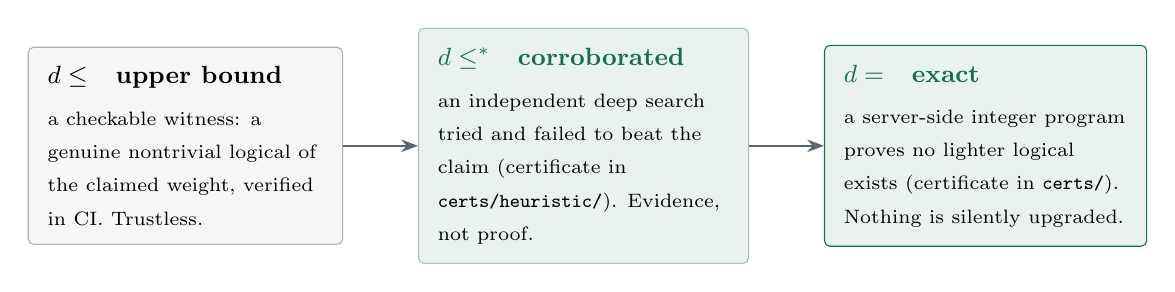
\begin{tikzpicture}[
		tier/.style={rounded corners=2pt, inner sep=7pt},
		arr/.style={-{Stealth[length=6pt]}, thick, muted}]
		\node[tier, fill=paper, draw=muted!50] (ub) at (0,0)
			{\begin{minipage}{3.5cm}\raggedright
			{\bfseries\small $d\le$ \; upper bound}\\[3pt]
			{\scriptsize a checkable witness: a genuine nontrivial logical of
			 the claimed weight, verified in CI. Trustless.}\end{minipage}};
		\node[tier, fill=trustwash, draw=trust!40, right=0.95cm of ub] (corr)
			{\begin{minipage}{3.7cm}\raggedright
			{\color{trust}\bfseries\small $d\le^{*}$ \; corroborated}\\[3pt]
			{\scriptsize an independent deep search tried and failed to beat
			 the claim (certificate in \texttt{certs/heuristic/}). Evidence,
			 not proof.}\end{minipage}};
		\node[tier, fill=trustwash, draw=trust, right=0.95cm of corr] (ex)
			{\begin{minipage}{3.6cm}\raggedright
			{\color{trust}\bfseries\small $d=$ \; exact}\\[3pt]
			{\scriptsize a server-side integer program proves no lighter
			 logical exists (certificate in \texttt{certs/}). Nothing is
			 silently upgraded.}\end{minipage}};
		\draw[arr] (ub) -- (corr);
		\draw[arr] (corr) -- (ex);
	\end{tikzpicture}
	\caption{The distance-confidence ladder. Every tier is backed by an
	artifact in the repository: a witness inside the submission, a heuristic
	certificate, or an exact certificate.}
	\label{fig:tiers}
	\end{figure}

	\paragraph{Upper-bound tier (trustless, in CI).} The submitter's witness
	is checked exactly as in (V6). A valid witness proves
	$d_{\text{side}}\le\texttt{value}$; the board labels such a code $d\le$
	and lets anyone climb instantly, since the arithmetic is checked rather
	than trusted.

	\paragraph{The refutation gate (adversarial, in CI).} Every changed code
	faces independent bounded searches for a logical \emph{lighter} than the
	claim: a random-information-set (RIS) search (randomized distance estimation in
	the spirit of \texttt{QDistRnd}~\cite{pryadko2023qdistrnd}) and a
	syndrome-decoder (BP+OSD) search~\cite{roffe2020decoding} --- two
	genuinely different mechanisms. Budgets are
	adaptive: trials scale with $n$, and a code that would enter a cell's
	Pareto frontier faces a much deeper multi-seed battery than a dominated
	one, so over-claims pay extra scrutiny exactly where gaming would matter.
	Frontier claims additionally face an accelerated RIS pass (a bit-packed
	$\GF$ engine at roughly $150\times$ the baseline trial budget) that only
	\emph{proposes} candidates: a find counts as a refutation solely after
	the trusted verifier validates the witness, so the extra depth adds no
	trust surface. Any hit is a sound refutation --- it exhibits a checkable
	counterexample --- and fails the PR. The per-run seed is random by
	design, so an over-claim cannot be tuned to evade one fixed search; a
	weekly whole-board sweep re-runs the refutation with fresh seeds to
	accumulate coverage over time.

	\paragraph{Corroborated tier.} A maintainer-run deep search
	(\texttt{verify/heuristic\_certify.py}) that tries and fails to beat a
	claim writes a heuristic certificate; the board then shows $d\le^{*}$.
	This is evidence, not proof --- the label records exactly how hard the
	claim has been attacked.

	\paragraph{Exact tier (server-certified).} To upgrade a side to $d=$, a
	maintainer runs \texttt{verify/certify.py}, which proves no lighter
	nontrivial logical exists via a bounded integer program (scipy/HiGHS, no
	commercial solver). For each logical generator $t_L$ of the relevant type
	it asks whether a $v$ exists with
	\begin{equation}
		H v \equiv 0,\qquad \langle v,t_L\rangle\equiv 1 \pmod 2,\qquad
		\wt(v)\le \texttt{value}-1,
		\label{eq:milp}
	\end{equation}
	the mod-2 constraints linearized by integer slacks. If every generator on
	both sides is proven \emph{infeasible}, $d$ is exact; if a lighter
	logical is found, the claim is \emph{refuted}; if the solver hits its
	time limit, the side honestly remains an upper bound. A successful run
	writes a certificate to \texttt{certs/<slug>.json}, which is what
	upgrades a code's board label to $d=$. Exact records outrank equal
	upper-bound ones; nothing is ever silently upgraded.

	\section{Trust architecture and automated discovery}
	\label{sec:trust}

	Automated code discovery already works: LLM-guided evolutionary
	search~\cite{cruzbenito2026evolutionary}, reinforcement
	learning~\cite{he2025reinforcement}, and LLM-driven concept evolution
	over non-abelian families~\cite{liu2026concept} all produce candidate codes far faster than humans can referee them ---
	and an overstated distance is precisely their characteristic failure
	mode. Several of the board's current records were machine-discovered and
	are attributed to the producing model in their provenance. The pipeline
	is therefore built so that \emph{nothing a submission can contain is
	trusted}, which is what makes it usable as the verification harness of an
	autoresearch loop (Figure~\ref{fig:zones}):
	\begin{itemize}[nosep]
		\item \textbf{Scope separation.} A PR that adds code data may not
		touch the verifier, schema, workflows, or site builder
		(\texttt{check\_submission\_scope.py}); and for code PRs the entire
		judgment runs from the \emph{base-branch} checkout, so a submission
		cannot alter the code it is judged by.
		\item \textbf{Pinned validation stack.} The trusted closure --- the
		verifier, the refutation engine, the GF(2) core, the local
		\texttt{validate\_candidate} gate, and the integrity checker itself
		--- is pinned by a SHA-256 manifest; any drift fails CI, and
		re-pinning is a deliberate, reviewable act.
		\item \textbf{Authorship binding.} The PR author must be a listed
		author of the codes they add
		(\texttt{check\_authorship.py}).
		\item \textbf{Duplicate fingerprints.} The reduced-row-echelon forms
		of $(\HX,\HZ)$ pin the exact stabilizer group --- an identical
		fingerprint is a hard CI error --- and a permutation-invariant
		Weisfeiler--Leman signature on the Tanner graph flags possible
		equivalents for human review.
		\item \textbf{Local gate for agents.} An autoresearch agent may
		explore freely, but by convention (\texttt{research/AUTORESEARCH.md})
		no code is a find until the pinned \texttt{validate\_candidate}
		returns \texttt{passed:\,true} --- the same verdict CI will reach,
		computable before a PR is ever opened.
	\end{itemize}

	\section{Repository layout and automation}

	\begin{center}
		\begin{tabular}{ll}
			\toprule
			Path & Contents\\
			\midrule
			\texttt{schema/}   & submission format (JSON Schema + \texttt{SCHEMA.md})\\
			\texttt{verify/}   & the trusted stack (\texttt{gf2.py},
			                     \texttt{qldpc\_verify.py},
			                     \texttt{heuristic\_distance.py},\\
			                   & \texttt{validate\_candidate.py}, all
			                     hash-pinned); the CI gates
			                     (\texttt{gate\_changed.py},\\
			                   & scope, authorship, integrity); the offline
			                     tiers (\texttt{certify.py},\\
			                   & \texttt{heuristic\_certify.py}); an optional
			                     C++ search accelerator; tests\\
			\texttt{decode/}   & the BP+OSD syndrome-decoder cross-check\\
			\texttt{codes/}    & accepted submissions and seeded baselines
			                     (the board data)\\
			\texttt{certs/}    & exact and heuristic distance certificates\\
			\texttt{research/} & contributor tooling: family samplers and
			                     screening kit, the\\
			                   & open-boundary planar engine, and the
			                     autoresearch agent manual\\
			\texttt{site/}     & \texttt{build.py}, which generates the static site\\
			\texttt{docs/}     & the generated site (index, per-code pages,
			                     references, badges)\\
			\texttt{cli/}      & \texttt{./qldpc submit}: matrices in,
			                     verified PR-ready JSON out\\
			\texttt{TRACKS.md} & the three ranking layers and how cells work\\
			\bottomrule
		\end{tabular}
	\end{center}
	CI (\texttt{.github/workflows/verify.yml}) runs, in order: the scope
	check, the validator-integrity check, the convention-discovered
	self-tests, \texttt{verify\_all.py} over every board code, the refutation
	gate on the changed codes, and the authorship check. A separate weekly
	workflow re-attacks the whole board with fresh seeds
	(\texttt{refute-weekly.yml}), and the site workflow rebuilds
	\texttt{docs/} on every push to \texttt{main}. The badges and figures are
	regenerated from the live board on every build, so they track the current
	numbers rather than a hand-typed count.

	\paragraph{State of the board.} At the time of writing the board holds 48
	verified codes --- 26 submitted through the challenge and 22 literature
	baselines, 29 of them certified exact --- across the bivariate-bicycle,
	generalized-bicycle (including non-abelian two-block group-algebra),
	coset, tile, and topological families. Recent machine-discovered entries
	illustrate the intended dynamics: a $[[336,20,20]]$ two-block code on
	$\mathrm{PSL}(2,7)$ (the Klein-quartic group) currently carries the
	board's best $\eff = 23.81$; a $[[240,13,15]]$ code on the symmetric
	group $S_5$ is the board's first odd-$k$ entry (odd $k$ is impossible for
	abelian two-block constructions); and a $[[216,15,11]]$ grafted planar
	bilayer code leads the 2D-local weight-8 cell. Each survived the same
	discipline the gate enforces --- deep multi-seed self-refutation before
	submission, with witnesses validated by the pinned stack --- and in one
	recent agent-driven sweep, five of seven staged frontier candidates were
	refuted \emph{before} submission. The live figures are in
	\texttt{docs/stats.json}.

	\section{Open questions this could surface}

	\begin{itemize}[nosep]
		\item Can planar (open-boundary) codes close the efficiency gap to
		the periodic and unrestricted records, or is part of the gap
		intrinsic to boundaries?
		\item How far does the non-abelian two-block design space reach?
		Groups outside the systematically enumerated ranges --- the board's
		$\mathrm{PSL}(2,7)$ and $S_5$ entries are first examples --- keep
		yielding record parameters.
		\item How deep must a refutation search run before an upper-bound
		claim at a given $n$ deserves confidence? The board's history,
		including refutations of its own staged candidates, is a growing
		dataset on exactly this question.
		\item Can the exact-certification tier scale past $n\approx 300$,
		where the integer programs currently time out?
	\end{itemize}

	{\small
	\bibliographystyle{unsrt}
	\bibliography{../refs}
	}

\end{document}
